\documentclass[/home/jesse/Analysis/FemtoAnalysis/AnalysisNotes/AnalysisNoteJBuxton.tex]{subfiles}
\begin{document}

\subsubsection{V0 Purity Background Estimation}
\label{V0PurBgdEst}

As previously stated, the backgrounds in the \minv distributions are modeled by a polynomial which is fit outside of the final cut region in an attempt to estimate the background within the cut region.  
As this estimate of the background under the mass peak is vital for our estimate of our V0 purity, it is important for us to ensure that our estimate is accurate.  
More specifically, it is necessary that we ensure the background is well described by a polynomial fit within the cut region.

To better understand our background, we studied V0 candidates reconstructed with daughters from different events.  
These mixed-event V0s certainly do not represent real, physical V0s (a single V0 cannot have daughters living in two different events!), but, rather, represent a large portion of the background creeping into our analysis.

The standard AliFemto framework is not equipped to handle this situation, as most are not interested in these fake-V0s.  
Therefore, we built a new class, AliFemtoV0PurityBgdEstimator, to handle our needs.  
In addition to finding fake-V0s using mixed-event daughters, we also used our new class to find real-V0s using same-event daughters.  
The purpose here was to compare our new class to the established V0 finder used in standard AliFemto analyses.


\begin{figure}[h!]
  \centering
  %%----start of first subfigure---  
  \subfloat[\Ks]{
    \label{fig:V0PurBgdEst:a}
    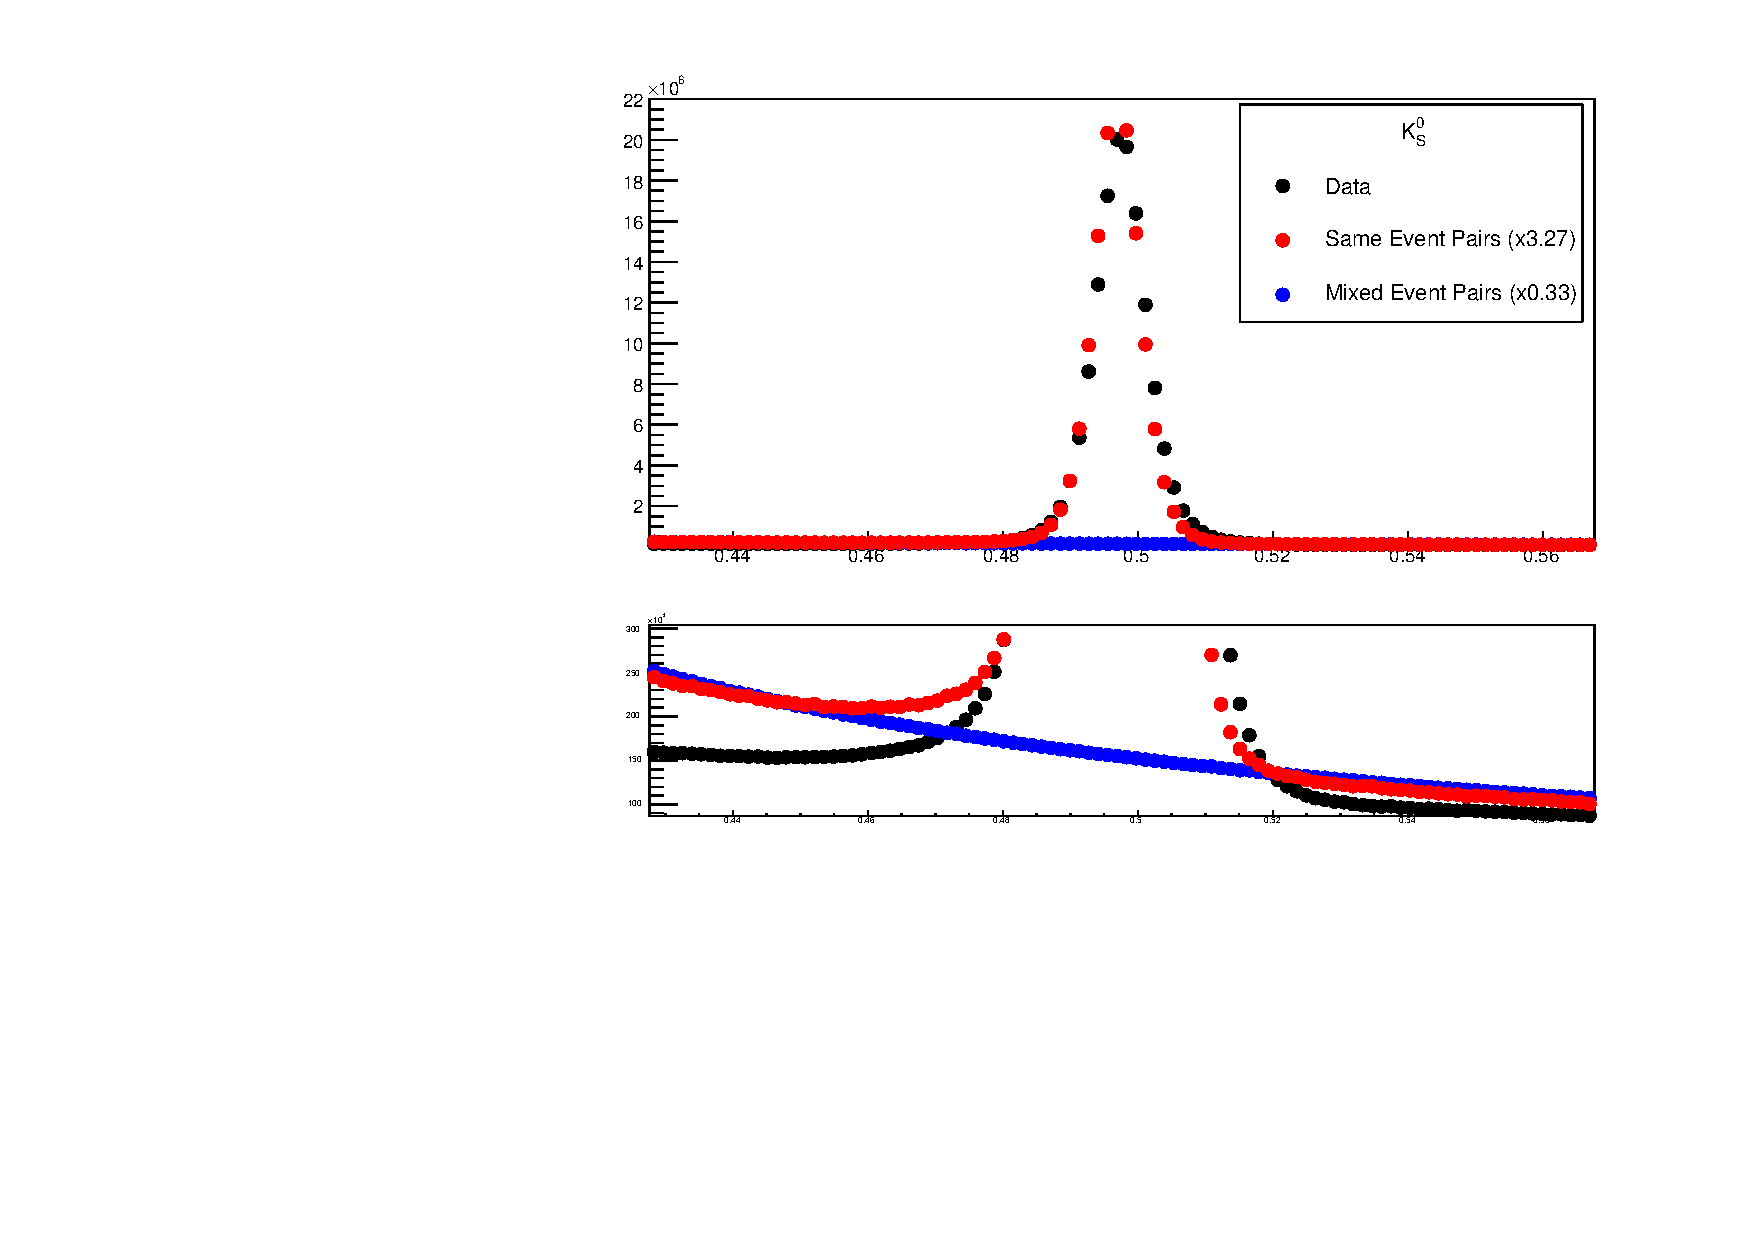
\includegraphics[width=0.49\textwidth]{/home/jesse/Analysis/FemtoAnalysis/AnalysisNotes/3_DataSelection/Figures/V0PurBgdEst_DataVsNumVsDenK0.pdf}}
  %%----start of second subfigure---
  \subfloat[\Lam]{
    \label{fig:V0PurBgdEst:b}
    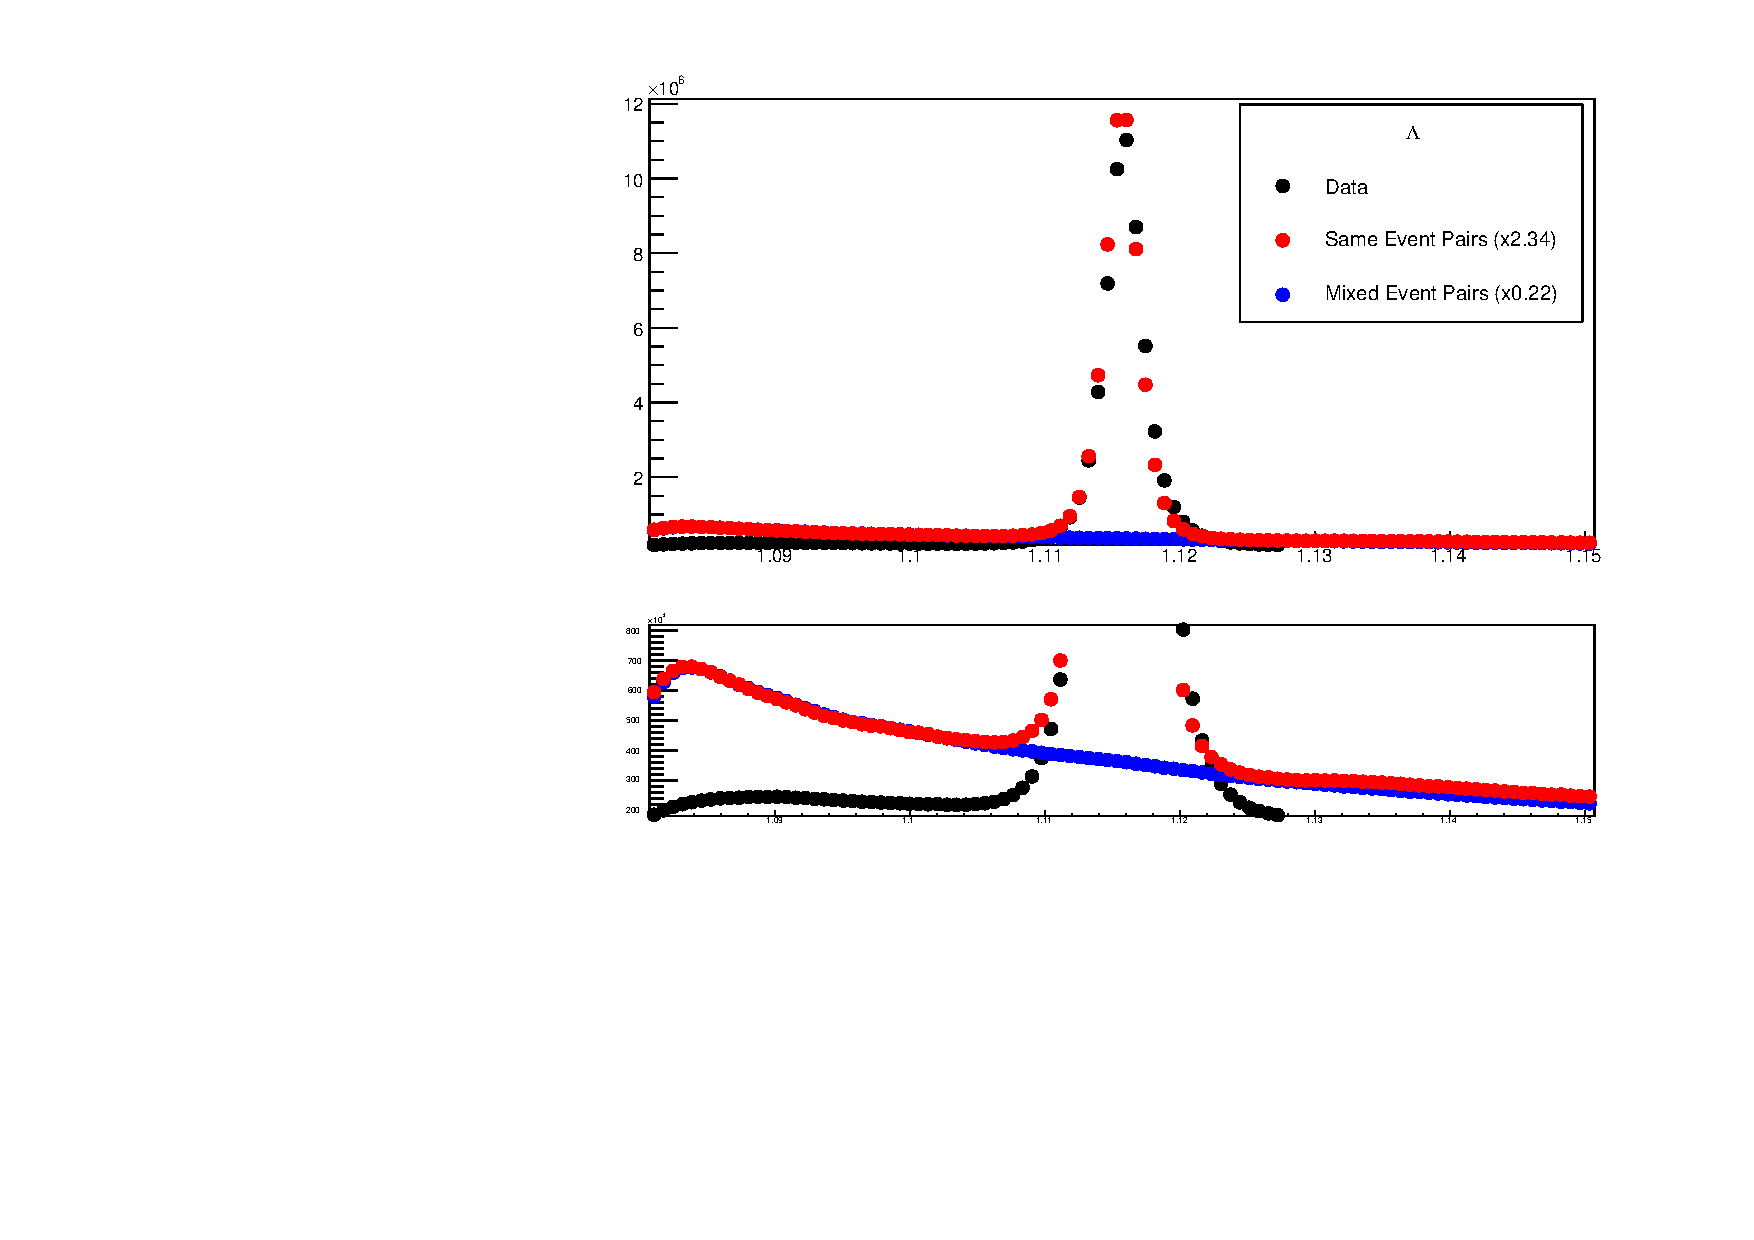
\includegraphics[width=0.49\textwidth]{/home/jesse/Analysis/FemtoAnalysis/AnalysisNotes/3_DataSelection/Figures/V0PurBgdEst_DataVsNumVsDenLam.pdf}}
  %%----overall caption----
  \caption[V0 Purity Background Estimation]
  {
  V0 Purity Background Estimation.  
  The black points, marked ``Data", correspond to real V0s found using the standard V0-finder (i.e. the V0s used in my analyses).  
  The red points, marked ``Same Event Pairs", show real V0s reconstructed with our personal V0-finder in AliFemtoV0PurityBgdEstimator.
  These data are scaled by a factor (listed in the legend) to match their $Signal+Background$ value in the cut region with that of the data.  
  The blue points, marked ``Mixed Event Pairs", show fake-V0s reconstructed with our personal V0-finder using mixed-event daughters.  
  The blue points are scaled by a factor (listed in the legend) to closely match the red points in the side-band region.
  }
  \label{fig:V0PurBgdEst}
\end{figure}

Figure \ref{fig:V0PurBgdEst} shows the results of our study.  
In the figures, the black points, marked ``Data", correspond to V0s found using the standard V0-finder, and to the V0s used in my analyses.
The red and blue points utilize our personal V0-finder (i.e. AliFemtoV0PurityBgdEstimator).
The red points show real V0s reconstructed using same-event daughters, and the blue points show fake-V0s reconstructed using mixed-event daughters.  
Both the red and blue points have been scaled by different factors (listed in the legends) to nicely align all three data on a single plot.

Figure \ref{fig:V0PurBgdEst} shows that our personal V0-finder does a good, but not perfect, job of matching the shape of the $m_{\mathrm{inv}}$ plots obtained from the data.  
The scale factor listed in the legend reveals that we are only finding ~1/3 - 1/2 of the V0s found by the standard V0-finder.  
These two points are not of concern, as our purpose here was to gain a sense of the broad shape of the background.  
It is revealed in Fig. \ref{fig:V0PurBgdEst}, when studying the red and blue points, that the background distribution within the mass peak region is simply a smooth connection of the backgrounds outside of the cut region, as we assumed.  
Therefore, our method of fitting the background outside of the cut region, fitting with a smooth polynomial, and extrapolating to the cut region is justified.


\end{document}